\setcounter{definition}{0} \setcounter{property}{0} \setcounter{claim}{0} \setcounter{fact}{0} \setcounter{corollary}{0} \setcounter{figure}{0}

\section{Fast Fourier Transform~(FFT)}

The Fourier Transform is a fundamental technique with critical applications in
signal processing and many others. It appears
in various forms across different domains, but all share the same
algorithmic core. In this class, we study its version in polynomials.

\subsection*{Evaluation and Interpolation}

Let's start with lines~(polynomial of degree 1).
A line is described using its function $y(x) = a_0 + a_1 x$.
It is uniquely determined by the two coefficients $a = (a_0, a_1)$.
A line can also be determined by \emph{any} two \emph{distinct} points on it: $(x_0, y_0)$ and $(x_1, y_1)$.
The process that computes $y_0$ and $y_1$ given $a$ and the chosen $x_0$ and $x_1$
is called \emph{evaluation}. The opposite process, that computes $a$ from $(x_0, y_0)$ and $(x_1, y_1)$
is called \emph{interpolation}.

Evaluation can be written in matrix form 
\[
\begin{bmatrix} y_0 \\ y_1 \end{bmatrix}
=
\begin{bmatrix} 1 & x_0 \\ 1 & x_1 \end{bmatrix}
\cdot
\begin{bmatrix} a_0 \\ a_1 \end{bmatrix},
\]
whereas interpolation can be written as 
\[
\begin{bmatrix} a_0 \\ a_1 \end{bmatrix}
=
\begin{bmatrix} 1 & x_0 \\ 1 & x_1 \end{bmatrix}^{-1}
\cdot
\begin{bmatrix} y_0 \\ y_1 \end{bmatrix}.
\]

Note that matrix $[ 1\ x_0; 1\ y_0]$ is invertible if and only if $x_0 \neq x_1$, verifying
two \emph{distinct} points determine the line. The explicit form of the inverse is
\[
\begin{bmatrix} 1 & x_0 \\ 1 & x_1 \end{bmatrix}^{-1}
=
\frac{1}{x_1 - x_0}
\begin{bmatrix} x_1 & -x_0 \\ -1 & 1 \end{bmatrix}.
\]

We now generalize above definitions to higher-order polynomials.
Let 
\[ y(x) = a_0 + a_1 x + a_2 x^2 + \cdots a_{n-1} x^{n-1}\] % = \sum_{j=0}^{n-1} a_j x^j\]
be a polynomial of degree $n-1$.
Similarly, $y(x)$ is also uniquely determined by $n$ distinct points on it, namely
$\{(x_0,y_0), (x_1, y_1), \cdots, (x_{n-1}, y_{n-1})\}$, where $x_i \neq x_j$, $0 \le i < j \le n-1$,
and $y_j = y(x_j)$, $j = 0, 1, 2, \cdots, n-1$.
The evaluation is written as:
\[
\begin{bmatrix} y_0 \\ y_1 \\ y_2 \\ \vdots \\ y_{n-1} \end{bmatrix}
=
\begin{bmatrix}
1 & x_0 & x_0^2 & \cdots & x_0^{n-1} \\
1 & x_1 & x_1^2 & \cdots & x_1^{n-1} \\
1 & x_2 & x_2^2 & \cdots & x_2^{n-1} \\
\vdots & \vdots & \vdots & \ddots & \vdots \\
1 & x_{n-1} & x_{n-1}^2 & \cdots & x_{n-1}^{n-1}
\end{bmatrix}
\cdot
\begin{bmatrix} a_0 \\ a_1 \\ a_2 \\ \vdots \\ a_{n-1} \end{bmatrix},
\]
which we simplify as
\[ y = M \cdot a.  \]
The matrix $M$, parameterized by $(x_0, x_1, \cdots, x_{n-1})$, is called the Vandermonde matrix.

The interpolation is therefore
\[ a = M^{-1} \cdot y.  \]
The Vandermonde matrix $M$ is invertible if and only if $x_i \neq x_j$ for all $0 \le i < j \le n-1$, 
verifying that $n$ \emph{distinct} points fully determine the polynomial.

We aim for designing fast algorithms for evaluation and interpolation~(i.e., fast fourier transform).


\subsection*{Algorithm for Evaluation}

%Let's start with evaluation. 
For any choice of $n$ values $(x_0, x_1, \cdots, x_{n-1})$, 
one can compute $y_j = y(x_j) = a_0 + a_1x_j + a_2x_j^2 + \cdots + a_{n-1} x_j^{n-1}$ in $\Theta(n)$ time,
simply following the function, for each $j$. Hence, this straitforward approach takes $\Theta(n^2)$ time
to evaluate all $\{x_j\}$, $j = 0, 1, \cdots, n-1$.

We now design an $\Theta(n\log n)$ time algorithm, using the divide-and-conquer technique, for evaluation.
One of the key points for achieving a faster algorithm is the careful choice of $\{x_j\}$.
Again, as long as these values are distinct, they uniquely determine the polynomial. 
The right choice of $\{x_j\}$ is the $n$ roots of $x^n = 1$. Note that $x^n = 1$ has $n$ distinct roots
in complex plane. 

\begin{figure}[h!]
\centering{\tikzset{every picture/.style={line width=0.75pt}} %set default line width to 0.75pt        

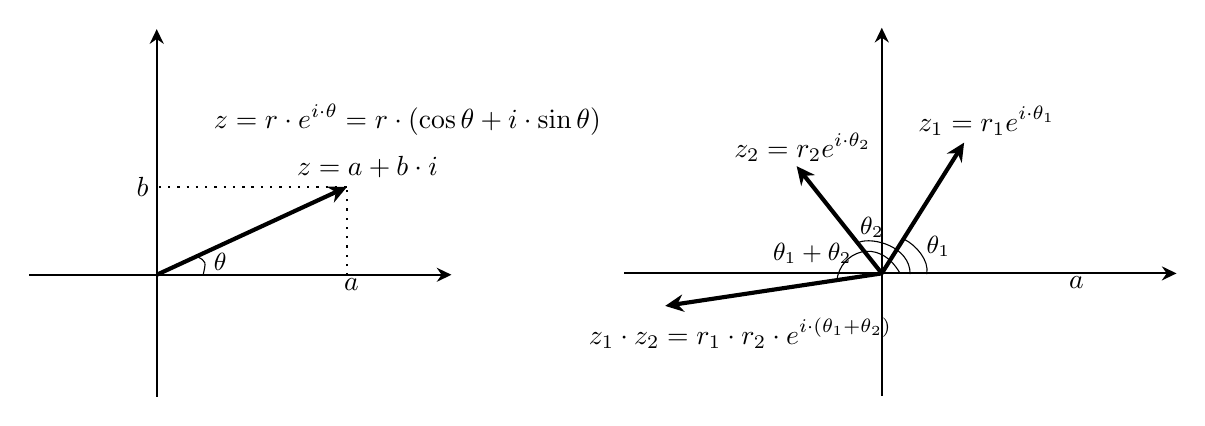
\begin{tikzpicture}[x=0.5pt,y=0.5pt,yscale=-1,xscale=1]
%uncomment if require: \path (0,313); %set diagram left start at 0, and has height of 313

%Straight Lines [id:da8759123208415905] 
\draw [color={rgb, 255:red, 0; green, 0; blue, 0 }  ,draw opacity=1 ][line width=0.75]    (330.52,214.5) -- (28,214.5) ;
\draw [shift={(333.52,214.5)}, rotate = 180] [fill={rgb, 255:red, 0; green, 0; blue, 0 }  ,fill opacity=1 ][line width=0.08]  [draw opacity=0] (10.72,-5.15) -- (0,0) -- (10.72,5.15) -- (7.12,0) -- cycle    ;
%Straight Lines [id:da821272442788836] 
\draw [color={rgb, 255:red, 0; green, 0; blue, 0 }  ,draw opacity=1 ][line width=0.75]    (120.52,40) -- (120.52,303) ;
\draw [shift={(120.52,37)}, rotate = 90] [fill={rgb, 255:red, 0; green, 0; blue, 0 }  ,fill opacity=1 ][line width=0.08]  [draw opacity=0] (10.72,-5.15) -- (0,0) -- (10.72,5.15) -- (7.12,0) -- cycle    ;
%Straight Lines [id:da671644264403058] 
\draw [color={rgb, 255:red, 0; green, 0; blue, 0 }  ,draw opacity=1 ][line width=1.5]    (254.37,152.68) -- (120.52,214.5) ;
\draw [shift={(258,151)}, rotate = 155.21] [fill={rgb, 255:red, 0; green, 0; blue, 0 }  ,fill opacity=1 ][line width=0.08]  [draw opacity=0] (13.4,-6.43) -- (0,0) -- (13.4,6.44) -- (8.9,0) -- cycle    ;
%Straight Lines [id:da23468734573164285] 
\draw [color={rgb, 255:red, 0; green, 0; blue, 0 }  ,draw opacity=1 ][line width=0.75]  [dash pattern={on 0.84pt off 2.51pt}]  (258,215) -- (258,151) ;
%Straight Lines [id:da9615311619238165] 
\draw [color={rgb, 255:red, 0; green, 0; blue, 0 }  ,draw opacity=1 ][line width=0.75]  [dash pattern={on 0.84pt off 2.51pt}]  (122,151) -- (258,151) ;
%Straight Lines [id:da7684706213932966] 
\draw [color={rgb, 255:red, 0; green, 0; blue, 0 }  ,draw opacity=1 ][line width=0.75]    (854.52,213.5) -- (458,213.5) ;
\draw [shift={(857.52,213.5)}, rotate = 180] [fill={rgb, 255:red, 0; green, 0; blue, 0 }  ,fill opacity=1 ][line width=0.08]  [draw opacity=0] (10.72,-5.15) -- (0,0) -- (10.72,5.15) -- (7.12,0) -- cycle    ;
%Straight Lines [id:da6533221507591959] 
\draw [color={rgb, 255:red, 0; green, 0; blue, 0 }  ,draw opacity=1 ][line width=0.75]    (644.52,39) -- (644.52,302) ;
\draw [shift={(644.52,36)}, rotate = 90] [fill={rgb, 255:red, 0; green, 0; blue, 0 }  ,fill opacity=1 ][line width=0.08]  [draw opacity=0] (10.72,-5.15) -- (0,0) -- (10.72,5.15) -- (7.12,0) -- cycle    ;
%Straight Lines [id:da054729749207868106] 
\draw [color={rgb, 255:red, 0; green, 0; blue, 0 }  ,draw opacity=1 ][line width=1.5]    (701.87,122.39) -- (644.52,213.5) ;
\draw [shift={(704,119)}, rotate = 122.19] [fill={rgb, 255:red, 0; green, 0; blue, 0 }  ,fill opacity=1 ][line width=0.08]  [draw opacity=0] (13.4,-6.43) -- (0,0) -- (13.4,6.44) -- (8.9,0) -- cycle    ;
%Straight Lines [id:da37945188035781485] 
\draw [color={rgb, 255:red, 0; green, 0; blue, 0 }  ,draw opacity=1 ][line width=1.5]    (585.49,139.13) -- (644.52,213.5) ;
\draw [shift={(583,136)}, rotate = 51.56] [fill={rgb, 255:red, 0; green, 0; blue, 0 }  ,fill opacity=1 ][line width=0.08]  [draw opacity=0] (13.4,-6.43) -- (0,0) -- (13.4,6.44) -- (8.9,0) -- cycle    ;
%Curve Lines [id:da5454872321119888] 
\draw    (149,201) .. controls (157,205) and (156,205) .. (154,215) ;
%Curve Lines [id:da27173222922396245] 
\draw    (661,189) .. controls (669,193) and (679,204) .. (677,214) ;
%Curve Lines [id:da2426367815741498] 
\draw    (628,191) .. controls (638,187) and (665,194) .. (665,214) ;
%Straight Lines [id:da5276650115271059] 
\draw [color={rgb, 255:red, 0; green, 0; blue, 0 }  ,draw opacity=1 ][line width=1.5]    (491.96,236.41) -- (644.52,213.5) ;
\draw [shift={(488,237)}, rotate = 351.46] [fill={rgb, 255:red, 0; green, 0; blue, 0 }  ,fill opacity=1 ][line width=0.08]  [draw opacity=0] (13.4,-6.43) -- (0,0) -- (13.4,6.44) -- (8.9,0) -- cycle    ;
%Curve Lines [id:da6762459778146103] 
\draw    (612,219) .. controls (614,198) and (642,186) .. (657.76,213.5) ;

% Text Node
\draw (220,127) node [anchor=north west][inner sep=0.75pt]   [align=left] {$\displaystyle z=a+b\cdot i$};
% Text Node
\draw (254,215) node [anchor=north west][inner sep=0.75pt]   [align=left] {$\displaystyle a$};
% Text Node
\draw (104,142) node [anchor=north west][inner sep=0.75pt]   [align=left] {$\displaystyle b$};
% Text Node
\draw (160,197) node [anchor=north west][inner sep=0.75pt]  [font=\small] [align=left] {$\displaystyle \theta $};
% Text Node
\draw (669,91) node [anchor=north west][inner sep=0.75pt]   [align=left] {$\displaystyle z_{1} =r_{1} e^{i\cdot \theta _{1}}$};
% Text Node
\draw (778,214) node [anchor=north west][inner sep=0.75pt]   [align=left] {$\displaystyle a$};
% Text Node
\draw (675,185) node [anchor=north west][inner sep=0.75pt]  [font=\small] [align=left] {$\displaystyle \theta _{1}$};
% Text Node
\draw (431,244) node [anchor=north west][inner sep=0.75pt]   [align=left] {$\displaystyle z_{1} \cdot z_{2} =r_{1} \cdot r_{2} \cdot e^{i\cdot ( \theta _{1} +\theta _{2})}$};
% Text Node
\draw (627,171) node [anchor=north west][inner sep=0.75pt]  [font=\small] [align=left] {$\displaystyle \theta _{2}$};
% Text Node
\draw (160,89) node [anchor=north west][inner sep=0.75pt]   [align=left] {$\displaystyle z=r\cdot e^{i\cdot \theta } =r\cdot (\cos \theta +i\cdot \sin \theta )$};
% Text Node
\draw (536,110) node [anchor=north west][inner sep=0.75pt]   [align=left] {$\displaystyle z_{2} =r_{2} e^{i\cdot \theta _{2}}$};
% Text Node
\draw (564,190) node [anchor=north west][inner sep=0.75pt]  [font=\small] [align=left] {$\displaystyle \theta _{1} +\theta _{2}$};


\end{tikzpicture}

}
\caption{Illustration of complex numbers and their multiplication.}
\label{fig:complex}
\end{figure}

A complex number $z$ looks like $z = a + b\cdot i$, where $a$ is the real part and $b$ is the imaginary part.
It corresponds to a point in the complex plane with coordinates $(a, b)$, 
where its horizontal axis vertical axis represents the real part and imaginary part respectively.
See Figure~\ref{fig:complex}.

One of the nice thing about complex numbers are their polar form. 
A complex number $z = a+ b\cdot i$ can also be written as $z = r\cdot e^{i\cdot \theta}$,
where $r$ is the modulus of $z$, defined as $r = |z| = \sqrt{a^2 + b^2}$,
and $\theta$ is the angle between (the vector of) $z$ and the positive real axis.
This polar representation can be derived from the Euler’s identity: $e^{i\cdot \theta} = \cos \theta + i\cdot \sin \theta$.

Following the polar forms, the multiplication of two complex numbers can be done conveniently.
Let $z_1 = r_1\cdot e^{i\cdot \theta_1}$ and
$z_2 = r_2\cdot e^{i\cdot \theta_2}$. We have $z_1\cdot z_2 =r_1\cdot r_2 \cdot e^{i\cdot (\theta_1 + \theta_2)}$.
Geometrically, multiplication corresponds to rotation~(e.g., $\theta_1 + \theta_2$) and scaling~(e.g., $r_1\cdot r_2$).
See Figure~\ref{fig:complex}.


We now derive the roots of $x^n = 1$. Assume $x = r\cdot e^{i\cdot \theta}$.
We have $r^n \cdot e^{i\cdot \theta \cdot n} = r^n \cdot (\cos(\theta  n) + i\cdot \sin(\theta n)) = 1$.
We therefore must have $r^n = 1$ which gives $r = 1$, and $\theta n = 2\pi \cdot j$ for some non-negative integer $j$.
Hence, $\theta = 2 \pi / n \cdot j$. Picking $j = 0, 1, 2, \cdots, n - 1$ gives the $n$ distinct roots,
namely, 
\[  x_j = e^{2 \pi/ n \cdot j}, j = 0, 1, 2, \cdots, n-1. \]

\begin{figure}[t!]
\centering{

\tikzset{every picture/.style={line width=0.75pt}} %set default line width to 0.75pt        

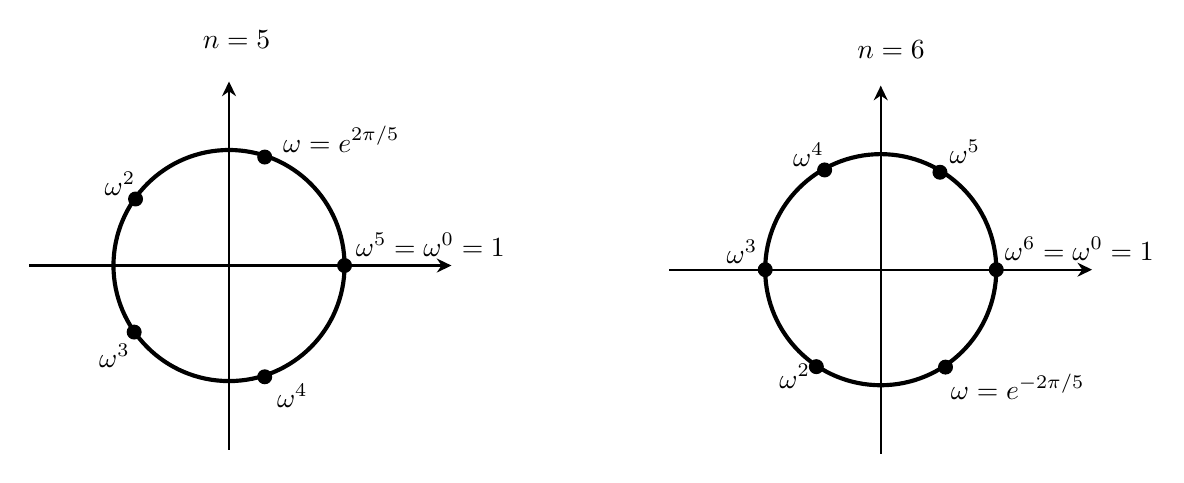
\begin{tikzpicture}[x=0.5pt,y=0.5pt,yscale=-1,xscale=1]
%uncomment if require: \path (0,445); %set diagram left start at 0, and has height of 445

%Straight Lines [id:da8759123208415905] 
\draw [color={rgb, 255:red, 0; green, 0; blue, 0 }  ,draw opacity=1 ][line width=0.75]    (338.52,214.5) -- (36,214.5) ;
\draw [shift={(341.52,214.5)}, rotate = 180] [fill={rgb, 255:red, 0; green, 0; blue, 0 }  ,fill opacity=1 ][line width=0.08]  [draw opacity=0] (10.72,-5.15) -- (0,0) -- (10.72,5.15) -- (7.12,0) -- cycle    ;
%Straight Lines [id:da821272442788836] 
\draw [color={rgb, 255:red, 0; green, 0; blue, 0 }  ,draw opacity=1 ][line width=0.75]    (180.76,84.5) -- (180.76,347.5) ;
\draw [shift={(180.76,81.5)}, rotate = 90] [fill={rgb, 255:red, 0; green, 0; blue, 0 }  ,fill opacity=1 ][line width=0.08]  [draw opacity=0] (10.72,-5.15) -- (0,0) -- (10.72,5.15) -- (7.12,0) -- cycle    ;
%Shape: Circle [id:dp05681939794999513] 
\draw  [line width=1.5]  (97.26,214.5) .. controls (97.26,168.38) and (134.65,131) .. (180.76,131) .. controls (226.88,131) and (264.26,168.38) .. (264.26,214.5) .. controls (264.26,260.62) and (226.88,298) .. (180.76,298) .. controls (134.65,298) and (97.26,260.62) .. (97.26,214.5) -- cycle ;
%Shape: Circle [id:dp3013076520100272] 
\draw  [fill={rgb, 255:red, 0; green, 0; blue, 0 }  ,fill opacity=1 ] (259.26,214.5) .. controls (259.26,211.74) and (261.5,209.5) .. (264.26,209.5) .. controls (267.02,209.5) and (269.26,211.74) .. (269.26,214.5) .. controls (269.26,217.26) and (267.02,219.5) .. (264.26,219.5) .. controls (261.5,219.5) and (259.26,217.26) .. (259.26,214.5) -- cycle ;
%Shape: Circle [id:dp42532911487328906] 
\draw  [fill={rgb, 255:red, 0; green, 0; blue, 0 }  ,fill opacity=1 ] (201.56,136.09) .. controls (201.56,133.33) and (203.8,131.09) .. (206.56,131.09) .. controls (209.33,131.09) and (211.56,133.33) .. (211.56,136.09) .. controls (211.56,138.85) and (209.33,141.09) .. (206.56,141.09) .. controls (203.8,141.09) and (201.56,138.85) .. (201.56,136.09) -- cycle ;
%Shape: Circle [id:dp661891511194406] 
\draw  [fill={rgb, 255:red, 0; green, 0; blue, 0 }  ,fill opacity=1 ] (108.21,166.42) .. controls (108.21,163.66) and (110.45,161.42) .. (113.21,161.42) .. controls (115.97,161.42) and (118.21,163.66) .. (118.21,166.42) .. controls (118.21,169.18) and (115.97,171.42) .. (113.21,171.42) .. controls (110.45,171.42) and (108.21,169.18) .. (108.21,166.42) -- cycle ;
%Shape: Circle [id:dp1005434022322731] 
\draw  [fill={rgb, 255:red, 0; green, 0; blue, 0 }  ,fill opacity=1 ] (201.56,294.91) .. controls (201.56,292.15) and (203.8,289.91) .. (206.56,289.91) .. controls (209.33,289.91) and (211.56,292.15) .. (211.56,294.91) .. controls (211.56,297.67) and (209.33,299.91) .. (206.56,299.91) .. controls (203.8,299.91) and (201.56,297.67) .. (201.56,294.91) -- cycle ;
%Shape: Circle [id:dp9205997842787009] 
\draw  [fill={rgb, 255:red, 0; green, 0; blue, 0 }  ,fill opacity=1 ] (107.21,262.58) .. controls (107.21,259.82) and (109.45,257.58) .. (112.21,257.58) .. controls (114.97,257.58) and (117.21,259.82) .. (117.21,262.58) .. controls (117.21,265.34) and (114.97,267.58) .. (112.21,267.58) .. controls (109.45,267.58) and (107.21,265.34) .. (107.21,262.58) -- cycle ;
%Straight Lines [id:da5753672664447395] 
\draw [color={rgb, 255:red, 0; green, 0; blue, 0 }  ,draw opacity=1 ][line width=0.75]    (801.52,217.5) -- (499,217.5) ;
\draw [shift={(804.52,217.5)}, rotate = 180] [fill={rgb, 255:red, 0; green, 0; blue, 0 }  ,fill opacity=1 ][line width=0.08]  [draw opacity=0] (10.72,-5.15) -- (0,0) -- (10.72,5.15) -- (7.12,0) -- cycle    ;
%Straight Lines [id:da6881124738646721] 
\draw [color={rgb, 255:red, 0; green, 0; blue, 0 }  ,draw opacity=1 ][line width=0.75]    (651.76,87.5) -- (651.76,350.5) ;
\draw [shift={(651.76,84.5)}, rotate = 90] [fill={rgb, 255:red, 0; green, 0; blue, 0 }  ,fill opacity=1 ][line width=0.08]  [draw opacity=0] (10.72,-5.15) -- (0,0) -- (10.72,5.15) -- (7.12,0) -- cycle    ;
%Shape: Circle [id:dp5675892160974338] 
\draw  [line width=1.5]  (568.26,217.5) .. controls (568.26,171.38) and (605.65,134) .. (651.76,134) .. controls (697.88,134) and (735.26,171.38) .. (735.26,217.5) .. controls (735.26,263.62) and (697.88,301) .. (651.76,301) .. controls (605.65,301) and (568.26,263.62) .. (568.26,217.5) -- cycle ;
%Shape: Circle [id:dp7901124514711858] 
\draw  [fill={rgb, 255:red, 0; green, 0; blue, 0 }  ,fill opacity=1 ] (730.26,217.5) .. controls (730.26,214.74) and (732.5,212.5) .. (735.26,212.5) .. controls (738.02,212.5) and (740.26,214.74) .. (740.26,217.5) .. controls (740.26,220.26) and (738.02,222.5) .. (735.26,222.5) .. controls (732.5,222.5) and (730.26,220.26) .. (730.26,217.5) -- cycle ;
%Shape: Circle [id:dp8992653780362201] 
\draw  [fill={rgb, 255:red, 0; green, 0; blue, 0 }  ,fill opacity=1 ] (689.56,147.09) .. controls (689.56,144.33) and (691.8,142.09) .. (694.56,142.09) .. controls (697.33,142.09) and (699.56,144.33) .. (699.56,147.09) .. controls (699.56,149.85) and (697.33,152.09) .. (694.56,152.09) .. controls (691.8,152.09) and (689.56,149.85) .. (689.56,147.09) -- cycle ;
%Shape: Circle [id:dp7236067841601378] 
\draw  [fill={rgb, 255:red, 0; green, 0; blue, 0 }  ,fill opacity=1 ] (606.21,145.42) .. controls (606.21,142.66) and (608.45,140.42) .. (611.21,140.42) .. controls (613.97,140.42) and (616.21,142.66) .. (616.21,145.42) .. controls (616.21,148.18) and (613.97,150.42) .. (611.21,150.42) .. controls (608.45,150.42) and (606.21,148.18) .. (606.21,145.42) -- cycle ;
%Shape: Circle [id:dp5665363843506173] 
\draw  [fill={rgb, 255:red, 0; green, 0; blue, 0 }  ,fill opacity=1 ] (693.56,287.91) .. controls (693.56,285.15) and (695.8,282.91) .. (698.56,282.91) .. controls (701.33,282.91) and (703.56,285.15) .. (703.56,287.91) .. controls (703.56,290.67) and (701.33,292.91) .. (698.56,292.91) .. controls (695.8,292.91) and (693.56,290.67) .. (693.56,287.91) -- cycle ;
%Shape: Circle [id:dp7356242289210358] 
\draw  [fill={rgb, 255:red, 0; green, 0; blue, 0 }  ,fill opacity=1 ] (600.21,287.58) .. controls (600.21,284.82) and (602.45,282.58) .. (605.21,282.58) .. controls (607.97,282.58) and (610.21,284.82) .. (610.21,287.58) .. controls (610.21,290.34) and (607.97,292.58) .. (605.21,292.58) .. controls (602.45,292.58) and (600.21,290.34) .. (600.21,287.58) -- cycle ;
%Shape: Circle [id:dp22660151420836994] 
\draw  [fill={rgb, 255:red, 0; green, 0; blue, 0 }  ,fill opacity=1 ] (563.26,217.5) .. controls (563.26,214.74) and (565.5,212.5) .. (568.26,212.5) .. controls (571.02,212.5) and (573.26,214.74) .. (573.26,217.5) .. controls (573.26,220.26) and (571.02,222.5) .. (568.26,222.5) .. controls (565.5,222.5) and (563.26,220.26) .. (563.26,217.5) -- cycle ;

% Text Node
\draw (160,43) node [anchor=north west][inner sep=0.75pt]   [align=left] {$\displaystyle n=5$};
% Text Node
\draw (633,50) node [anchor=north west][inner sep=0.75pt]   [align=left] {$\displaystyle n=6$};
% Text Node
\draw (218,112) node [anchor=north west][inner sep=0.75pt]   [align=left] {$\displaystyle \omega =e^{2\pi /5}$};
% Text Node
\draw (89,145) node [anchor=north west][inner sep=0.75pt]   [align=left] {$\displaystyle \omega ^{2}$};
% Text Node
\draw (85,269) node [anchor=north west][inner sep=0.75pt]   [align=left] {$\displaystyle \omega ^{3}$};
% Text Node
\draw (213.56,297.91) node [anchor=north west][inner sep=0.75pt]   [align=left] {$\displaystyle \omega ^{4}$};
% Text Node
\draw (270.56,188.91) node [anchor=north west][inner sep=0.75pt]   [align=left] {$\displaystyle \omega ^{5} =\omega ^{0} =1$};
% Text Node
\draw (586.56,123.91) node [anchor=north west][inner sep=0.75pt]   [align=left] {$\displaystyle \omega ^{4}$};
% Text Node
\draw (538.56,193.91) node [anchor=north west][inner sep=0.75pt]   [align=left] {$\displaystyle \omega ^{3}$};
% Text Node
\draw (576.56,283.91) node [anchor=north west][inner sep=0.75pt]   [align=left] {$\displaystyle \omega ^{2}$};
% Text Node
\draw (699.56,121.91) node [anchor=north west][inner sep=0.75pt]   [align=left] {$\displaystyle \omega ^{5}$};
% Text Node
\draw (739.56,191.91) node [anchor=north west][inner sep=0.75pt]   [align=left] {$\displaystyle \omega ^{6} =\omega ^{0} =1$};
% Text Node
\draw (700.56,290.91) node [anchor=north west][inner sep=0.75pt]   [align=left] {$\displaystyle \omega =e^{-2\pi /5}$};


\end{tikzpicture}

}
\caption{Roots of $x^n = 1$ on complex plane, where $\omega$ denotes a primitive.}
\label{fig:roots}
\end{figure}

Geometrically, these $n$ roots locate evenly along the unit circle of the complex plane.
See Figure~\ref{fig:roots}.
A root is called \emph{primitive}, if its powers generates all $n$ roots.
Clearly, $x_1 = e^{2\pi/n}$ is a primitive, as $\{x_1^j\}$, $j = 0, 1, \cdots, n-1$,
is exactly the set of $n$ roots. It is obvious that 
$x_{n-1} = e^{2\pi/n\cdot (n-1)} = e^{-2\pi/n}$ is also a primitive.
Note that not every root is a primitive.
We use $\omega$ to represent a primitive; again 
$\{\omega^j\}$, $j = 0, 1, \cdots, n-1$, gives all the $n$ roots.

The evaluation task now becomes, given $y(x)$ represented using $a = (a_0, a_1, \cdots, a_{n-1})$ and a primitive $\omega$,
to compute $y(\omega^j)$, for $j =0, 1, \cdots, n-1$. In matrix form, it is to compute $M(\omega) \cdot a$, where 
\[
M(\omega) =
\begin{bmatrix}
1 & 1 & 1 & \cdots & 1 \\
1 & \omega^1 & \omega^2 & \cdots & \omega^{n-1} \\
1 & \omega^2 & \omega^4 & \cdots & \omega^{2(n-1)} \\
\vdots & \vdots & \vdots & \ddots & \vdots \\
1 & \omega^{n-1} & \omega^{2(n-1)} & \cdots & \omega^{(n-1)\cdot(n-1)}
\end{bmatrix}.
\]
We define a recursive function, called FFT($a = (a_0, \cdots, a_{n-1}), \omega$), that returns
$(y(\omega^0), y(\omega^1), \cdots, y(\omega^{n-1}))$ stored in a vector $T$ of size $n$.

To design the (divide-and-conquer) algorithm, we first re-write $y(x)$ by separating even and odd terms.
Assume that $n$ is even.
\begin{align*}
y(x) & = a_0 + a_1x + a_2 x^2 + \cdots + a_{n-2} x^{n-2} + a_{n-1} x^{n-1} \\
& = \left(a_0 + a_2 x^2 + a_4x^4 + \cdots + a_{n-2} x^{n-2} \right) + \left(a_1x + a_3 x^3 + a_5 x^5 + \cdots + a_{n-1} x^{n-1} \right) \\
& = \left(a_0 + a_2 x^2 + a_4x^4 + \cdots + a_{n-2} x^{n-2} \right) + x\cdot \left(a_1 + a_3 x^2 + a_5 x^4 + \cdots + a_{n-1} x^{n-2} \right).
\end{align*}
Define
\begin{align*}
y_e(x) &= a_0 + a_2 x + a_4 x^2 + \cdots + a_{n-2} x^{(n-2)/2},  \\
y_o(x) &= a_1 + a_3 x + a_5 x^2 + \cdots + a_{n-1} x^{(n-2)/2},
\end{align*}
where both $y_e(x)$ and $y_o(x)$ are degree of $(n-2)/2$, we can re-write $y(x)$ as
\[ y(x) = y_e(x^2) + x\cdot y_o(x^2). \]

Note that if $\omega$ is a primitive of $x^n = 1$, then $\omega^2$ must be a primitive of $x^{n/2} = 1$. (Can you prove it?)
Then it is valid to call FFT($a_0, a_2, \cdots, a_{n-2}, \omega^2)$ and FFT($a_1, a_3, \cdots, a_{n-1}, \omega^2)$, 
as suggested by above rewriting.

Let's carefully work out what these two calls return, following the definition of FFT.
The first call evaluates $y(x) = a_0 + a_2 x + a_4 x^2 + \cdots + a_{n-2} x^{(n-2)/2}$ which is \emph{exactly} $y_e(x)$.
So it returns $y_e(\omega^{2j})$, for $j=0, 1, \cdots, (n-2)/2$, stored in a vector which we call $T_e$, of size $n/2$.
Similary, the second call evaluates
$y(x) = a_1 + a_3 x + a_5 x^2 + \cdots + a_{n-1} x^{(n-2)/2}$ which is \emph{exactly} $y_o(x)$,
and it therefore returns $y_o(\omega^{2j})$, for $j=0, 1, \cdots, (n-2)/2$, stored in a vector which we call $T_o$, of size $n/2$.

It should be clear now that above two recursive calls offers exactly what we need to compute 
\[  y(\omega^j) = y_e(\omega^{2j}) + \omega \cdot y_o(\omega^{2j}), j = 0, 1, 2, \cdots, n-1. \]
But be careful that both $T_o$ and $T_e$ is of size $n/2$, i.e., they store $y_e(\omega^{2j})$ and
$y_o(\omega^{2j})$ for $j$ up to $(n-2)/2$. Good news is that, when $j \ge n/2$, we
have $\omega^{2j} = \omega^{2j-n}$ since $\omega^n = 1$.
\textcolor{blue}{Hence, when $j\ge n/2$, we have $y_e(\omega^{2j}) = y_e(\omega^{2j-n}) = T_e[j-n/2]$
and $y_o(\omega^{2j}) = y_o(\omega^{2j-n}) = T_o[j-n/2]$.}

%% The combining step, which returns the required vector $T$ of size $n$, can be computed as follows.\\
%% For $j = 0, 1, \cdots, (n-2)/2$: 
%% $$T[j] = y(\omega^j) = y_e(\omega^{2j}) + \omega \cdot y_o(\omega^{2j}) = T_e[j] + \omega \cdot T_o[j];$$
%% For $j = n/2, n/2+1, \cdots, n-1$: 
%% $$T[j] = y(\omega^j) = y_e(\omega^{2j}) + \omega \cdot y_o(\omega^{2j}) = 
%% y_e(\omega^{2j-n}) + \omega \cdot y_o(\omega^{2j-n}) = T_e[j-n/2] + \omega \cdot T_o[j-n/2].$$

The complete pseudo-code for evaluation is given below.

\begin{minipage}{0.8\textwidth}
        \aaA {11}{function FFT($a_0, a_1, \cdots, a_{n-1}, \omega$)}\xxx
        \aab {handle base case for $n \le 2$ and return as needed;}\xxx
        \aab {$T_e =$ FFT($a_0, a_2, \cdots, a_{n-2}, \omega^2$)}\xxx
        \aab {$T_o =$ FFT($a_1, a_3, \cdots, a_{n-1}, \omega^2$)}\xxx
        \aaB {2}{for $j=0$ to $(n-2)/2$}\xxx
		\aac {$T[j] = y(\omega^j) = y_e(\omega^{2j}) + \omega \cdot y_o(\omega^{2j}) = T_e[j] + \omega \cdot T_o[j]$;}\xxx
%        \aac {$T[j] = T_e[j] + \omega\cdot T_o[j]$;}\xxx
        \aab {end}\xxx
        \aaB {2}{for $j=n/2+1$ to $n-1$}\xxx
		\aac {$T[j] = y(\omega^j) = y_e(\omega^{2j}) + \omega \cdot
			y_o(\omega^{2j}) = y_e(\omega^{2j-n}) + \omega \cdot
				y_o(\omega^{2j-n}) = T_e[j-n/2] + \omega \cdot T_o[j-n/2]$;} \xxx
        %\aac {$T[j] = T_e[j-n/2] + \omega\cdot T_o[j-n/2]$;}\xxx
        \aab {end}\xxx
        \aab {return $T$}\xxx
        \aaa {end algorithm;}\xxx
\end{minipage}

Above algorithm clearly runs in $\Theta(n\log n)$ time.


\subsection*{Algorithm for Interpolation}

It turns out that interpolation is very easy!
Recall that interpolations seeks to compute $M(\omega)^{-1} \cdot y$, where
$y = (y(\omega^0), y(\omega^1), \cdots, y(\omega^{n-1}))^T$.
Thanks to the special form of $M(\omega)$,
it is proved that
	   \[ M(\omega)^{-1} = 1/n \cdot M(\omega^{-1}).\]
This immediately gives an algorithm for interpolation: 
	$$a = M(\omega)^{-1} \cdot y = 1/n \cdot M(\omega^{-1}) \cdot y = 1/n \cdot \textrm{FFT}(y, \omega^{-1}) = 1/n \cdot \textrm{FFT}(y(\omega^0), y(\omega^1), \cdots, y(\omega^{n-1}), \omega^{-1}).$$
Again, since $\omega$ is a primitive of $x^n=1$, $\omega^{-1}$ must be also a primitive of $x^n=1$.
Therefore above call to function FFT is valid.

\subsection*{An Application: Polynomial Multiplication}

The problem is, given $A(x) = a_0 + a_1x + a_2x^2 + \cdots + a_{n-1} x^{n-1}$ and
$B(x) = b_0 + b_1x + b_2x^2 + \cdots + b_{n-1}x^{n-1}$, to compute $C(x) = A(x) \cdot B(x)$.
Both $A(x)$ and $B(x)$ are polynomials of degree $n-1$; hence $C(x)$ is a polynomial of degree $2n-2$.
Assume that $C(x) = c_0 + c_1x + c_2x^2 + \cdots + c_{2n-2}x^{2n-2}$. 
We have $c_0 = a_0b_0$, $c_1 = a_0b_1 + a_1b_0$, $c_2 = a_0b_2+ a_1b_1 + a_2b_0$, and so on.
Generally, $c_k = \sum_{i + j = k, i \ge 0, j\ge 0} a_ib_j$.
A naive way of computing $c_k$ following this equation takes $\Theta(n)$ time; hence
the total runtime of computing $C(x)$, i.e., computing $\{c_k\}$ for $k=0, 1, \cdots, 2n-2$, takes $\Theta(n^2)$ time.

Interestingly, above problem can be solved in $\Theta(n\log n)$ time using FFT!
In order to reconstruct $C(x)$, a polynomial of degree $2n-2$, we (only) need to
compute $C(\omega^j)$, $j = 0, 1, \cdots, 2n-2$, followed by the interpolation,
where $\omega$ is a primitive of $x^{2n-1} = 1$.
($\omega = e^{i\cdot 2\pi / (2n-1)}$ or $\omega = e^{-i\cdot 2\pi / (2n-1)}$ will work.)
Since $C(x) = A(x)\cdot B(x)$, computing $C(\omega^j)$, for all $j=0, 1, \cdots, 2n-2$, will
take $\Theta(n)$ time, provided that $A(\omega^j)$ and $B(\omega^j)$ are known for all $j=0, 1, \cdots, 2n-2$.
These values can be obtained by evaluating $A(x)$ and $B(x)$. Since $\omega$ is a primitive of higher order,
we can rewrite $A(x) = a_0 + a_1x + \cdots a_{n-1}x^{n-1} + 0\cdot x^n + \cdots + 0\cdot x^{2n-2}$ and
$B(x) = b_0 + b_1x + \cdots b_{n-1}x^{n-1} + 0\cdot x^n + \cdots + 0\cdot x^{2n-2}$ as polynomials of degree of $2n-2$,
and then call FFT.  The complete pseudo-code is given below. It clearly runs in $\Theta(n\log n)$ time.

\begin{minipage}{0.8\textwidth}
        \aaA {10}{function polynomial-multiplication($a=(a_0, a_1, \cdots, a_{n-1}), b=(b_0, b_1, \cdots, b_{n-1})$)}\xxx
        \aab {let $\omega = e^{i\cdot 2\pi/(2n-1)}$}\xxx
        \aab {let $a' = (a_0, a_1, \cdots, a_{n-1}, 0, 0, \cdots, 0)$, by appending $n-1$ 0s to $a$;}\xxx
        \aab {let $b' = (b_0, b_1, \cdots, b_{n-1}, 0, 0, \cdots, 0)$, by appending $n-1$ 0s to $b$;}\xxx
        \aab {$Y_A =$ FFT($a', \omega$)}\xxx
        \aab {$Y_B =$ FFT($b', \omega$)}\xxx
        \aaB {2}{for $j=0$ to $2n-1$}\xxx
        \aac {$Y_C[j] = Y_A[j] \cdot Y_B[j]$;}\xxx
        \aab {end}\xxx
        \aab {return $1/(2n-1) \cdot \textrm{FFT}(Y_C, \omega^{-1})$}\xxx
        \aaa {end algorithm}\xxx
\end{minipage}

Let $a=(a_0, a_1, \cdots, a_{n-1})$ and $b=(b_0, b_1, \cdots, b_{n-1})$.
A new vector $c = (c_0, c_1, \cdots, c_{2n-2})$ defined using $c_k = \sum_{i + j = k, i \ge 0, j \ge 0} a_ib_j$,
is called the \emph{convolution} of $a$ and $b$.  Computing the convolution of two vectors
is equivalent to multiplying two polynomials, which can be done in $\Theta(n\log n)$ time using above algorithm.
